\section{Evaluation}
\subsection{Metrics and Methods of Experiment}
The metric of our experiments is time. The independent variable in this experiment is the number of nodes. We change the number of data nodes with different methods to compare the operation time. The experiments are divided into two parts, as one part is for measuring the encoding time of different methods, the other part is for timing the decoding time of different methods. The unit of the time is micro-second.\par

There are mainly two ways to compare different methods. One is for comparing the operational time of AP code with different parameters and that of one different method as we augment the number of data nodes. The other is for a general comparison with five data nodes for the encoding time, the decoding time in one disk, the decoding time in two disks and the decoding time in three disks for every method with its different parameters.\par

The environment of our experiment is listed below………….////////\par


\subsection{Numerical Results of Mathematical Analysis}
\subsubsection{Encoding Time Analysis}
From the Figure xx a), we could find out that the AP code encodes largely faster than RS ($k$, $3$). The rate of optimisation between AP($k$, $1$, $6$) and RS ($k$, $3$) is from 976.4\% (3 nodes’ case) to 849.2\% (13 nodes’ case), as the encoding time of AP codes multiplies about 4.7 times and that of RS code multiplies about 4.2 times. The Figure xx b) and c) illustrate that the effet of Star code and Tip code is similar, and the difference between them and AP code is not very large. The rate of optimisation between AP ($k$, $1$, $6$) and Star ($k$, $3$) is from 125.6\% (3 nodes’ case) to 127.3\% (17 nodes’ case). According to Figure xx d), we could see that AP code largely reduces the encoding time, comparing to LRC method. The rate of optimisation between AP code (k, 1, 4) and LRC (4k, 2, 4) is from 596.0\% (3 nodes’ case) to 615.8\% (13 nodes’ case); and the rate of optimisation between AP code ($k$, $1$, $6$) and LRC ($6k$, $2$, $6$) is from 684.0\% to 443.1\%. Considering the optimisation rate, AP code ($k$, $1$, $4$) is the best among the four.\par
\begin{figure}[H]
\begin{minipage}{0.25\lineWidth}
\centering
\includegraphics{Example1Modi2.jpg}
\caption{Encoding Time Comparison between AP method and RS method}
\end{minipage}
\begin{minipage}{0.25\lineWidth}
\centering
\includegraphics{Example2Modi1.jpg}
\caption{Encoding Time Comparison between AP method and Star method}
\end{minipage}
\begin{minipage}{0.25\lineWidth}
\centering
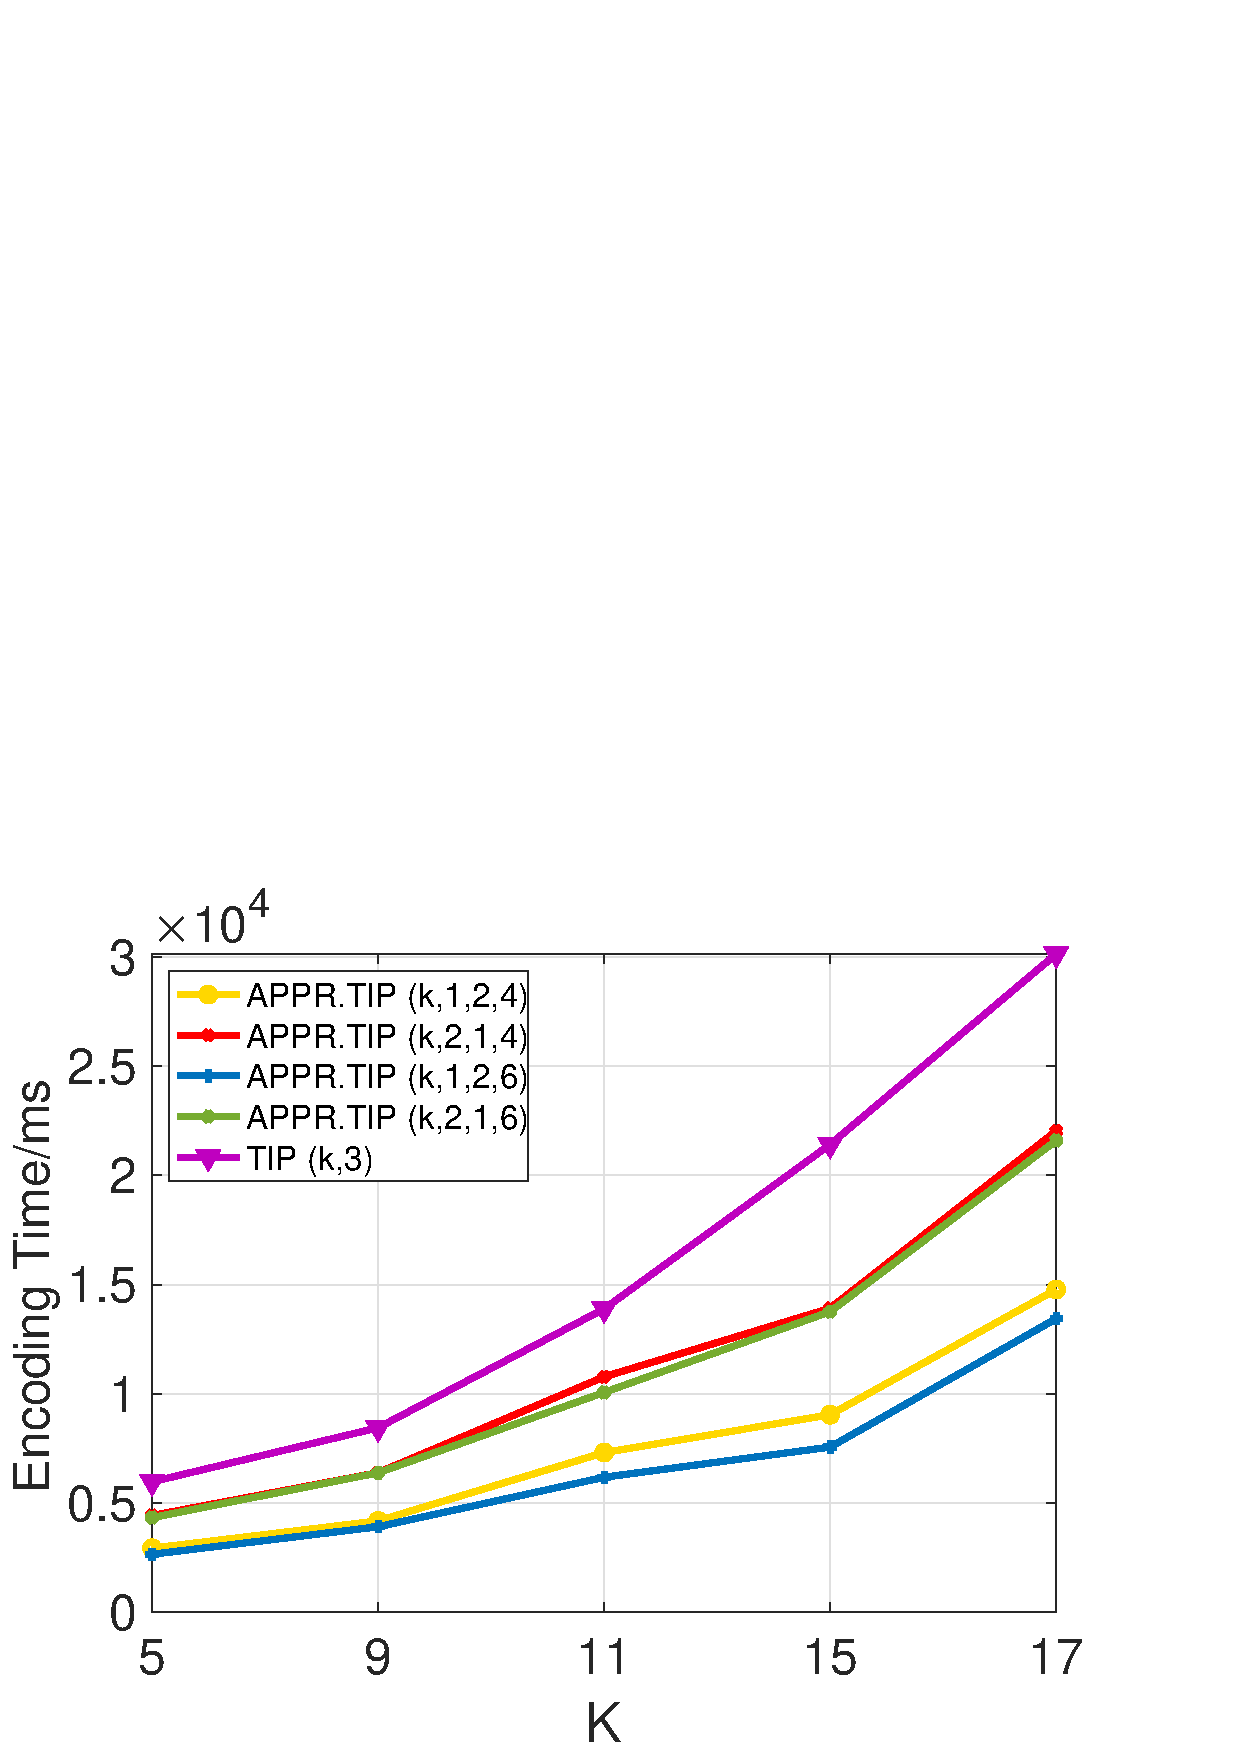
\includegraphics{Example3.jpg}
\caption{Encoding Time Comparison between AP method and Tip method}
\end{minipage}
\begin{minipage}{0.25\lineWidth}
\centering
\includegraphics{Example4.jpg}
\caption{Encoding Time Comparison between AP method and LRC method}
\end{minipage}
\end{figure}\par

According to Figure xx, we see that RS ($5$, $3$) has the longest encoding time among these methods, and the encoding time of LRC method is not short either. The methods whose encoding time is approaching to the AP method are Star and Tip. Among the AP method, AP ($5$, $1$, $6$) has the shortest encoding time.\par
\begin{figure}[H]
\centering
\includegraphics{BarEnT.jpg}
\caption{Comparison of Encoding Time for 5 Nodes with Different Methods}
\end{figure}

\subsubsection{Decoding Time in One Disk Analysis}
From the Figure xx a), we could find out that the AP code decodes faster than RS ($k$, $3$). The rate of optimisation between AP method ($k$, $1$, $6$) and RS ($k$, $3$) is from 395.2\% (3 nodes’ case) to 353.0\% (13 nodes’ case). The Figure xx b) and c) illustrate that the effet of Star code and Tip code is similar, and there is nearly no difference among these three methods. The rate of optimisation between AP method ($k$, $2$, $6$) and Star ($k$, $3$) is from 3.867\% (3 nodes’ case) to 2.971\% (17 nodes’ case). According to Figure xx d), we could see that LRC ($4k$, $2$, $4$) decodes a bit faster than AP code, but LRC ($6k$, $2$, $6$) decodes slower than AP code. LRC ($4k$, $2$, $4$) decodes faster from 5.941\% (3 nodes’ case) to 9.542\% (13 nodes’ case) than AP ($1$, $4$); but AP ($1$, $6$) decodes faster from 0.476\% (3 nodes’ case) to 6.196\% (13 nodes’ case) than LRC ($6k$, $2$, $6$).\par

\begin{figure}[H]
\begin{minipage}{0.25\lineWidth}
\centering
\includegraphics{Example5Modi1.jpg}
\caption{Decoding Time Comparison in One Disk between AP method and RS method}
\end{minipage}
\begin{minipage}{0.25\lineWidth}
\centering
\includegraphics{Example6.jpg}
\caption{Decoding Time Comparison in One Disk between AP method and Star method}
\end{minipage}
\begin{minipage}{0.25\lineWidth}
\centering
\includegraphics{Example7.jpg}
\caption{Decoding Time Comparison in One Disk between AP method and Tip method}
\end{minipage}
\begin{minipage}{0.25\lineWidth}
\centering
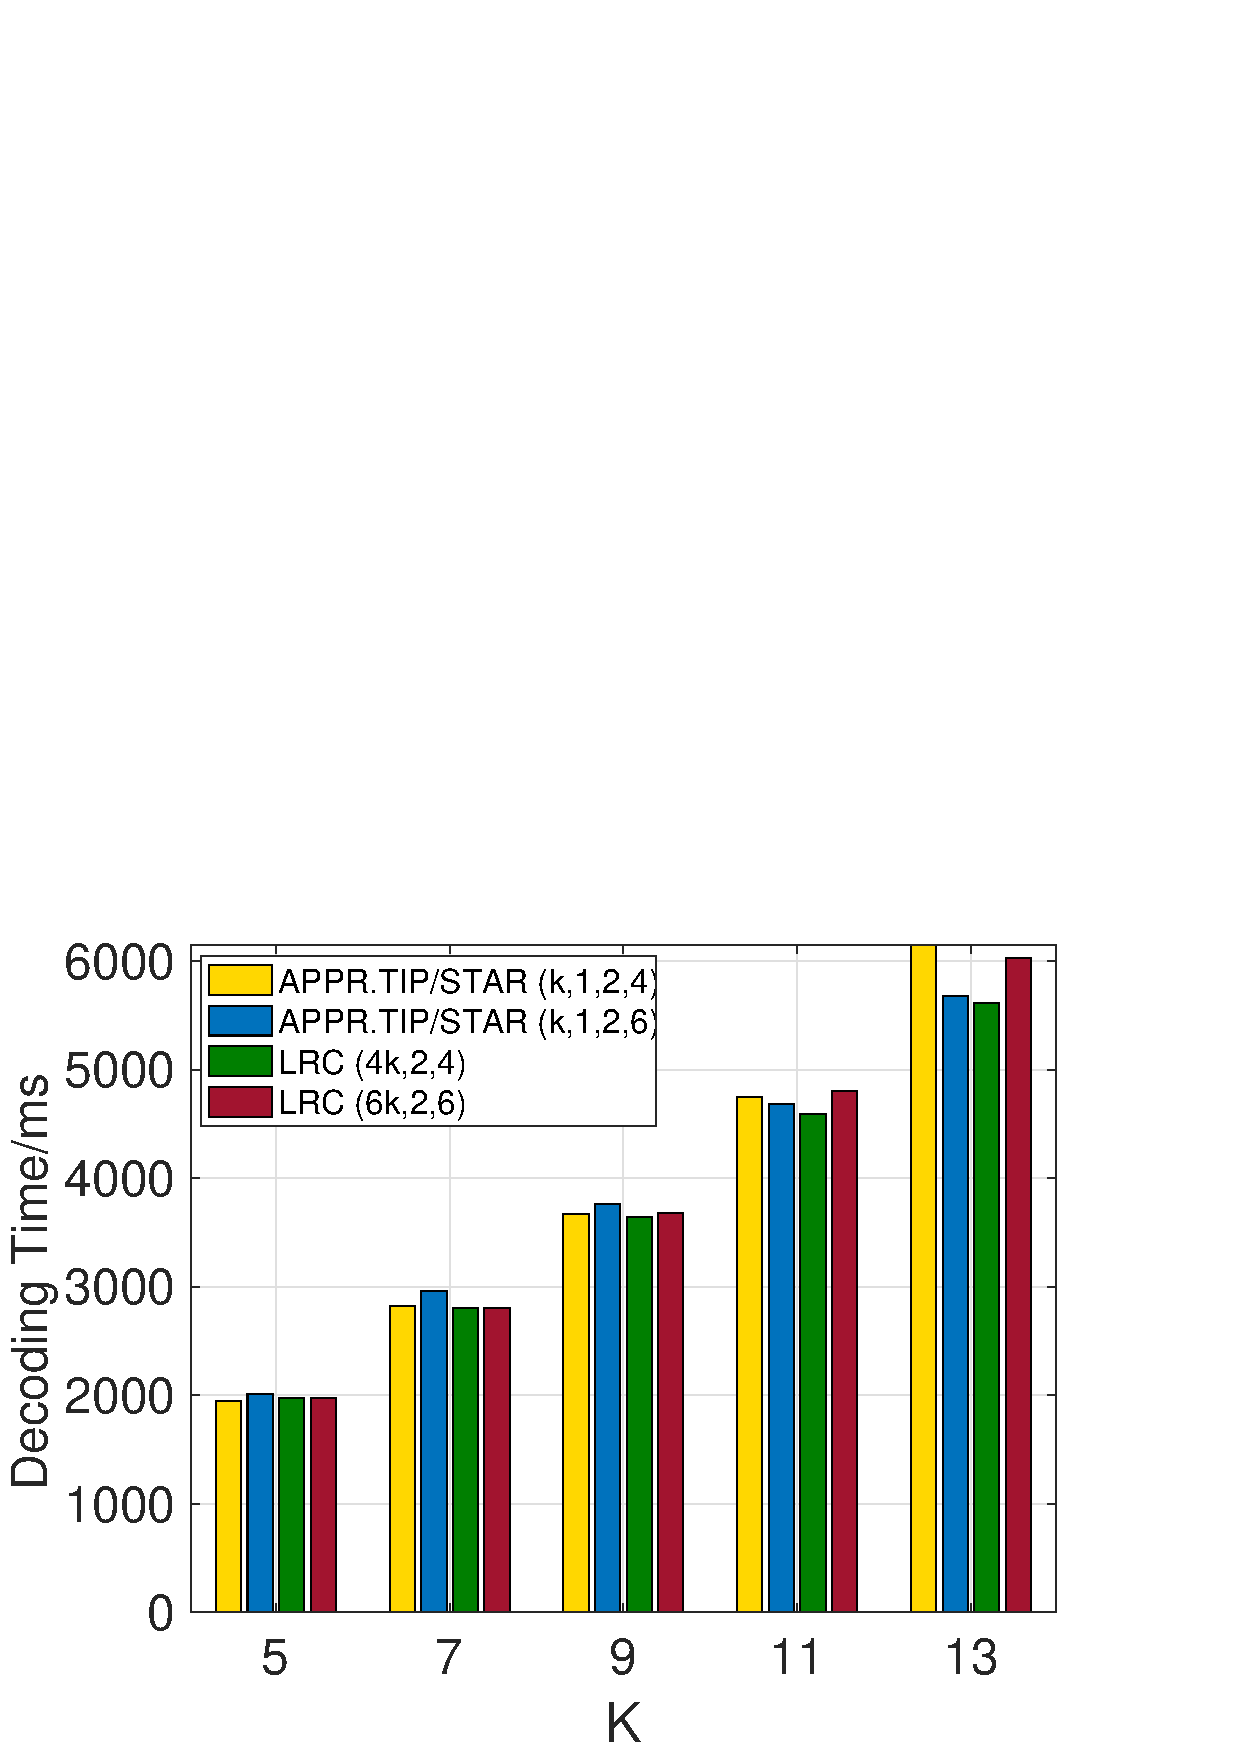
\includegraphics{Example8.jpg}
\caption{Decoding Time Comparison in One Disk between AP method and LRC method}
\end{minipage}
\end{figure}\par

According to Figure xx, we see that RS ($5$, $3$) has the longest decoding time among these methods, while other methods decoding time in one disk have no significant difference.\par
\begin{figure}[H]
\centering
\includegraphics{BarDeT1Modi1.jpg}
\caption{Comparison of Decoding Time for 5 Nodes in One Disk with Different Methods}
\end{figure}

\subsubsection{Decoding Time in Two Disks Analysis}
From the Figure xx a), we could find out that the AP code decodes remarkably faster than RS ($k$, $3$) in two disks. The rate of optimisation between AP method ($k$, $1$, $6$) and RS ($k$, $3$) is from 2782.1\% (3 nodes’ case) to 2593.9\% (13 nodes’ case). The Figure xx b) and c) illustrate that the effet of Star code and Tip code for decoding in two disks is similar, and the difference between them and AP ($k$, $2$, $4$ or $6$) is not very large. However, the difference is large when it comes to AP ($k$, $1$, $6$) The rate of optimisation between AP ($k$, $1$, $6$) and Star ($k$, $3$) is from 520.8\% (3 nodes’ case) to 508.6\% (17 nodes’ case). According to Figure xx d), we could see that AP code largely reduces the decoding time in two disks in comparison to LRC method. The rate of optimisation between AP code ($k$, $1$, $4$) and LRC ($4k$, $2$, $4$) is from 1971.5\% (3 nodes’ case) to 1265.5\% (13 nodes’ case); and the rate of optimisation between AP code ($k$, $1$, $6$) and LRC ($6k$, $2$, $6$) is from 2941.3\% to 1970.7\%. Considering the optimisation rate, AP code ($k$, $1$, $6$) is the best among the four.\par

\begin{figure}[H]
\begin{minipage}{0.25\lineWidth}
\centering
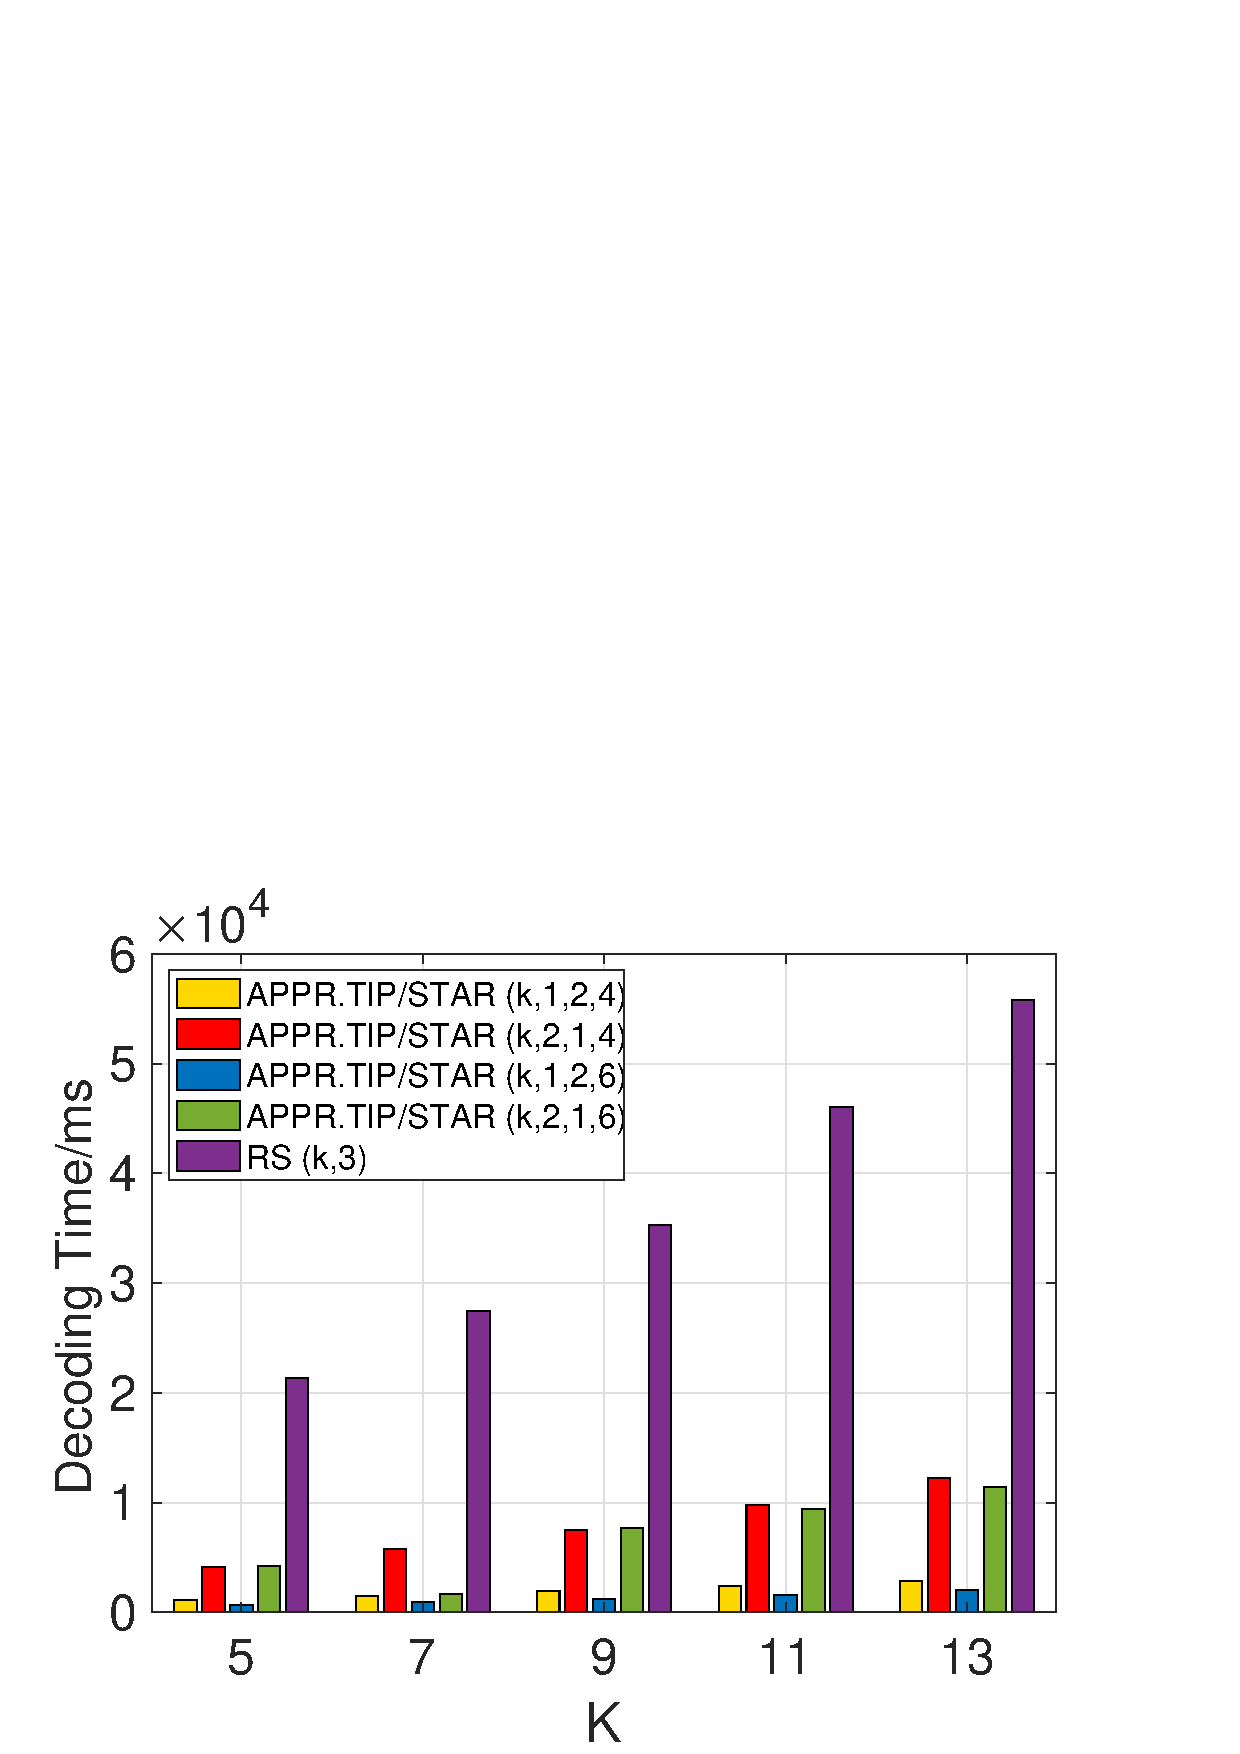
\includegraphics{Example9.jpg}
\caption{Decoding Time Comparison in Two Disks between AP method and RS method}
\end{minipage}
\begin{minipage}{0.25\lineWidth}
\centering
\includegraphics{Example10.jpg}
\caption{Decoding Time Comparison in Two Disks between AP method and Star method}
\end{minipage}
\begin{minipage}{0.25\lineWidth}
\centering
\includegraphics{Example11Modi1.jpg}
\caption{Decoding Time Comparison in Two Disks between AP method and Tip method}
\end{minipage}
\begin{minipage}{0.25\lineWidth}
\centering
\includegraphics{Example12.jpg}
\caption{Decoding Time Comparison in Two Disks between AP method and LRC method}
\end{minipage}
\end{figure}\par

According to Figure xx, we see that RS ($5$, $3$) has the longest decoding time among these methods, the LRC method is not suitable for decoding in two disks. AP code, here, largely reduces the decoding time in two disks, while the AP ($5$, $1$, $6$) keeps the shortest decoding time.
\begin{figure}[H]
\centering
\includegraphics{BarDeT2.jpg}
\caption{Comparison of Decoding Time for 5 Nodes in Two Disks with Different Methods}
\end{figure}
